\chapter{Do Your Own Research (DYOR)}
\label{ch:research}

Before you register for an exchange and rush in to get some cryptocurrency, it is vital to understand what you are purchasing. To comprehend what you are buying or supporting, you have to research the project in question and perform some due diligence.\medskip


\section{Action plan}
We advise you to take a holistic approach when it comes to your research. The story of Bitcoin and blockchain would be a great start for understanding the environment. For example, you might have heard about Bitcoin at some point and decided that it is time to read up on the subject and perhaps get some for yourself. In that case, you might want to start with the story of Bitcoin and blockchain technology which have severe implications for the future.

    \bigskip
    \begin{tipbox}{TIP}
    In \cref{app:A} you will find a wide range of sources (\cref{tab:research_data,tab:social_infrastructure,tab:marketinsight_analyses,tab:learning_tools_general,tab:security_tools}), that we've used over time to learn about Bitcoin, blockchain, cryptocurrency, money, and economics.
    \end{tipbox}
    \bigskip

Another example - and a logical next step - might be that you want to get involved with some of the alternative cryptocurrencies (altcoins) which are out there in droves. It is essential to understand that Bitcoin and blockchain are the fundamentals and it is crucial to understand these principles (at least in a general sense) before moving on to specific projects that involve cryptocurrency and are based on and make use of blockchain technology. Again, there is much information to be found on the subject of doing your research, which we will summarize in a concise checklist of elements. In \cref{app:A} you will find a broad range of tabulated resources (\cref{tab:research_data,tab:social_infrastructure,tab:marketinsight_analyses,tab:learning_tools_general,tab:security_tools}), in which we have documented some of the resources we have used in our research efforts. 

   

\section{Fundamental analysis}
\label{sec:fundamentalanalysis}

Typically, when investing in a company, fundamentals are key. The financial reports, the numbers, the performance of previous years and transparency are of vital importance to you being comfortable with your investments. Performing proper fundamental analysis of your prospective investments will drastically reduce your risk and will provide you with confidence regarding your own investment decisions.\medskip

When considering cryptocurrency and blockchain projects, which are still in their infancy stages, there are usually no financial reports, there is no track record of past performance, and many people base their decisions on speculation or hype. A company or corporation is centralized where a blockchain-based project can be designed fully decentralized. The community drives the development of these projects. You can consider the following elements when performing your fundamental analysis on your project of choice. From our own experience: it is effortless to get enthusiastic about a project which inevitably leads to forgetting to do your due diligence.

\begin{enumerate}
    \item \textbf{Technological Foundations}
    \begin{itemize}
        \item How strong or innovative is the technology?
        \item Are there bugs, network issues or vulnerabilities?
        \item How good is the codebase?
        \item What is the trade-off between speed, scalability, and security
    \end{itemize}
    \item \textbf{Usefulness}
    \begin{itemize}
        \item Short term utility? Long term utility?
        \item Does this project, and the corresponding token intend to solve a problem?
        \item Is it better than what we already have? Why?
        \item Is there a foreseeable demand for the token? Is it useful?
    \end{itemize}
    \item \textbf{Development Team}
    \begin{itemize}
        \item Does this project have a dedicated development team?
        \item How strong are their credentials? \item What is each member's previous experience? 
        \item Active contributions? Check commit history or activity on GitHub?
        \item How is the project funded?
    \end{itemize}
    \item \textbf{Community}
    \begin{itemize}
        \item Is there a passionate and friendly community behind the project?
        \item What is the level of activity in the community? How are people contributing?
    \end{itemize}
    \item \textbf{Governance}
    \begin{itemize}
        \item Is the project decentralized?
        \item Is the project open-source? Can you inspect the code for instance?
        \item Company funding, venture capital, foundation backing?
        \item Voting? Community influence?
    \end{itemize}
\end{enumerate}

How are you going to obtain all of this information? From what sources? For a total overview of the cryptocurrency market, we recommend starting at CoinMarketCap. This site provides information regarding the total market capitalization (and other metrics) of the cryptocurrency space and specifics on all of the enlisted projects. It also provides you with the links to the project website, social feeds, chats and source code. For fundamental analysis, the primary source of information is most likely the project's whitepaper, which is published by the development team. You will find the whitepapers on their respective websites. The whitepapers outline the vision, mission, problem statement and proposed solution and technical properties of the token or coin. In addition to the whitepaper, you should seek information regarding the level of activity of the developers and community. An excellent place to start would be the official social media and communication channels that the project has set up. You will find this information on the project website.

    \bigskip
    \begin{cryptobox}{\textbf{STATE OF THE DAPPS}}
        State of the DApps is a not-for-profit curated directory of Decentralized Applications, also called DApps, which run on various several blockchains. State of the DApps was initially created to categorize and showcase developed projects built on the Ethereum Blockchain, but more recently they have added support for EOS, POA and Steem as well. The inspiration for the State of the DApps came from FreshMeat, now known as FreeCode. FreeCode is a site reference for Linux users, which hosts a big inventory of the open source applications, games and all sources for Linux. In the State of the DApps there are many projects covering different fields such as health, games, virtual reality, artificial intelligence, education, registries, job markets, tinder for horses and many more. 
        \tcblower
        \href{https://www.stateofthedapps.com}{State of the DApps}; \textbf{Learn more about DApps}
    \end{cryptobox}
    \medskip

\subsection*{Project progression and development}
It is essential to follow the projects' progression to assess if they are taking their road-maps, timelines, and deadlines seriously and if they are transparent in their communication with the community. Other sources include community forums and video and blog sites. All these sources are a reliable way of obtaining diversified information and feedback from the community. Your effort stimulates the development of your understanding of what is going on with this particular project. You will spend quite some time reading or watching videos, but this is undoubtedly required and will aid you in developing your personal opinion and beliefs. Obtaining diverse information, which you have gathered yourself, based on your experience, forms a crucial part of your decision whether to invest or not.

    \bigskip
    \begin{tipbox}{\textbf{TIP}}
        The cryptocurrency world is alive on Twitter! There are plenty of alternatives, but Twitter is 'the place to be'. Do you want to stay up to date with the latest developments within the cryptocurrency environment? Be sure to follow us on Twitter.
        \tcblower
        \href{https://twitter.com/cryptomanuals}{Follow the Rabbit} op Twitter.
    \end{tipbox}

\section{Coin statistics}
Now that you have thoroughly investigated your potential future buy by doing your research as mentioned above, you could have a look at the statistics of the coin or token. Again, you will find many of these elements in the whitepaper, and usually, you will find at least some statistics and metrics while performing a certain degree of fundamental analysis. 

\begin{enumerate}
    \item \textbf{Supply}
    \begin{itemize}
        \item Capped or Uncapped? Circulating vs. Total Supply?
        \item Current Supply?
        \item Emission and Inflation?
        \item Distribution? Token Holders, Development Team, Marketing?
    \end{itemize}
    \item \textbf{Algorithm}
    \begin{itemize}
        \item Block Time and Confirmations
        \item Consensus Mechanism? Proof of Work, Proof of Stake or something complete else?
        \item ASIC Resistance?
    \end{itemize}
    \item \textbf{Market Capitalization, Trading Volume, and Liquidity}
    \begin{itemize}
        \item Check coin metrics on platforms such as listed in \cref{tab:marketinsight_analyses}
        \item Check ratios of Daily Trading Volume to Market Cap
    \end{itemize}
\end{enumerate}


\section{Technical analysis}
\label{sec:technicalanalysis}

Technical analysis is a trading tool employed to evaluate securities and identify trading opportunities by analyzing statistics gathered from trading activity, such as price movement and volume. Unlike fundamental analysts, who attempt to evaluate a security's intrinsic value, technical analysts focus on charts of price movement and various analytical tools to evaluate a security's strength or weakness. Technical analysts believe past trading activity, and price changes of securities are better indicators of their likely future price movements than the intrinsic value of the securities themselves. They think that the fundamental value is included in the stock or coin price.\medskip

Traders have many tools at their disposal provided by the technical analysis (TA), which can be used to analyze charts. Traders use technical analysis as a basis on which they time their buy and sell decisions. However, if you are not an experienced trader and have no clue what technical analysis is, you could learn the basics to prepare yourself with the knowledge to assess the optimal entry or exit point in this volatile market.

    \bigskip
        \begin{tipbox}{TIP}
        Learn more about the most popular trading-indicators such as the Bollinger Bands (BB), Relative Strength Index (RSI) and Moving Average Convergence Divergence (MACD) in \href{https://medium.com/@harrynicholls/7-popular-technical-indicators-and-how-to-use-them-to-increase-your-trading-profits-7f13ffeb8d05}{this article}.  
        \tcblower
        Go to \href{https://www.tradingview.com/}{TradingView} and add cryptocurrencies to your watchlist to track price movements.
        \end{tipbox}
    \medskip

There are several platforms you could use to have a go at technical analysis, and there are even platforms that provide you with several indexes and a whole bunch of aggregated services. \href{https://www.tradingview.com/}{TradingView} offers a platform to analyze charts of different markets which also hosts a community of active traders who post and share trading ideas. \href{https://coincheckup.com/}{CoinCheckUp} is a research platform which offers - among other things - different analysis methods and tools to help you get started. There are plenty more sources and platforms you could use, which we leave up to you to discover.

\section{Market psychology \& market sentiment}
The technical analysis aspects contribute to the economics of supply and demand at certain price levels of the (digital) asset. Market psychology and market sentiment also play a considerable part. The market for any (digital) asset consists of people, businesses and institutions from all over the world, all of which tend to behave both rational and irrational, and when markets move, emotions play a significant role. Recognizing this will be vital for success.\medskip

\begin{figure}
    \centering
    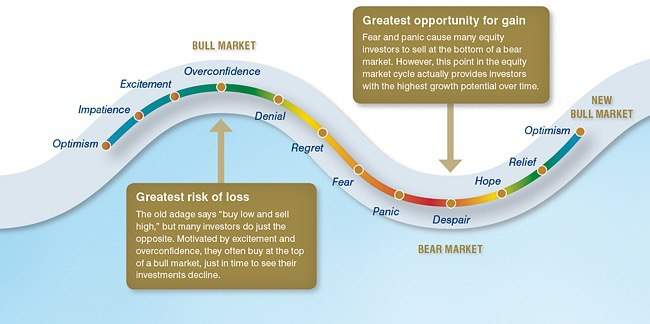
\includegraphics[width=.95\textwidth]{img/ch-investing/bear_bullmarket.jpg}
    \caption[Bear and Bull Markets and Market Psychology]{Market psychology is essentially what drives the so-called \say{bear} and \say{bull} markets. In every stage of the emotional cycle, there are decisions to be made by investors.}
    \label{fig:bear_bullmarket}
    \source{Brightscope; \textit{Research and Data.}}
\end{figure}

\medskip

\subsection{Bear markets}
When bear markets hit, there is fear, uncertainty, and doubt (FUD) and people tend to sell since the news is overwhelmingly negative. Bear markets can last for a very long time, which eliminates weak hands early on in the process. Furthermore, people who base their actions on what they see or hear usually failed to do fundamental research in the first place. In these scenarios, if you have performed your due diligence and feel confident about your previous investment decisions, you will have the strength to hold on for dear life (HODL). In other words, which enables you to ride out the storm and survive the potential onslaught of a cryptocurrency bear market. When sentiment is low, and selling seems to be the way to go - think again because it might be time to buy. If you didn't acquire any securities, stocks or coins, bear markets are an excellent time to consider entering the market, providing you to do the research. When timing buy-ins, technical analysis can come into play. You should feel more confident due to your fundamental analysis efforts and have just spotted an overall negative market sentiment. People are selling, as indicated by the price and chart movement.\medskip

\subsection{Bull markets}

When bull markets hit, there is a high degree of fear of missing out (FOMO), which can lead to overpriced stock. Trading volumes skyrocket and everybody seems to join in on the hype. Again, market sentiment and psychology play a huge role and are usually severely influenced by a torrent of positive news which creates a feedback loop. At the end of a bull run, the overpriced stocks plummet which may cause additional risk if you didn't time your exit point carefully.\medskip

\begin{figure}
    \centering
    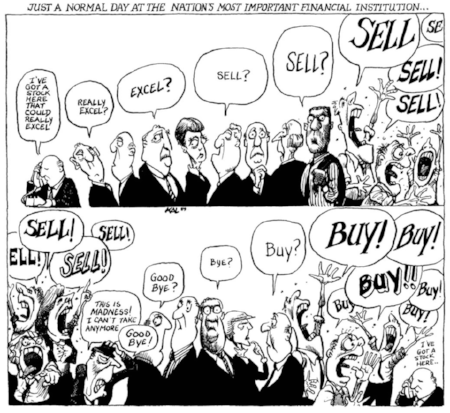
\includegraphics[width=.6\textwidth]{img/ch-investing/FOMOFUD.png}
    \caption{Fear, Uncertainty and Doubt (FUD) evolves into Fear Of Missing Out (FOMO).}
    \label{fig:FOMOFUD}
\end{figure}

\medskip

Keep in mind, the price is what you pay, and value is what you get $-$ pay too high a price, and returns are decimated. The value of a stock is relative to the number of earnings it will generate over the life of its business. In particular, this value is determined by discounting all future cash flows back to a present value, the intrinsic value. When you buy in too high (at unsustainable price levels) - the return that arises as an asset gravitates back to its intrinsic value over time will erode. Act greedy when others are fearful and reap enhanced profits. Explained; buy low, sell high and try to keep those emotions in check while making important decisions.\medskip 

\begin{tipbox}{\textbf{TIP}}
    Learn to control your emotions when making important decisions. Keep thinking critically, draw up a strategy, and be aware of the prevailing market sentiments and market psychology at the moment you decide to buy-in or buy-out.
\end{tipbox}



